\documentclass[usenames,dvipsnames,aspectratio=169]{beamer}
\usepackage[utf8]{inputenc}
\usepackage{xfrac}
\usepackage{amsmath}
\usepackage{graphicx}
\usepackage{dsfont}
\usepackage{apacite}
\usepackage{adjustbox}
\usepackage{booktabs}
\usepackage{amsfonts}
\usepackage{hyperref}
\usepackage{pdflscape}
\usepackage{lscape}
\usepackage{caption}
\usepackage{subcaption}
\usepackage{pgfplots}
\usepackage{xcolor}
\usepackage{epstopdf}
\usepackage{euler}
\usepackage{bbm}
\usepackage{multicol}
\usepackage{ulem}
\usepackage{cancel}
\usepackage{bbm}
\hypersetup{
    colorlinks,%
    citecolor=black,%
    filecolor=black,%
    linkcolor=black,%
    urlcolor=black
}   % useful for program listings
\usepackage{natbib}
\usecolortheme{seahorse}

\title{Leisure-Enhancing Technological Change  \\ \small{Applied Macroeconomics: Micro Data for Macro Models} }
\author{Author: Łukasz Rachel \\ 
Presented by: Jose M. Quintero}



\AtBeginSection[]
{
  \begin{frame}<beamer>
    \frametitle{Outline}
    \tableofcontents[currentsection]
  \end{frame}
}

\AtBeginSubsection[]
{
   \begin{frame}
        \frametitle{Outline}
        \tableofcontents[currentsubsection]
   \end{frame}
}



\begin{document}

\begin{frame}
  \titlepage
\end{frame}

\begin{frame}{Motivation}\label{p1:Int}
\begin{itemize}
    \item Leisure Enhancing Technologies (LET) have become increasingly relevant, and they differ from traditional products in the sense that \hyperlink{p1:Mot}{\beamerbutton{Trends}}
    \begin{enumerate}
        \item Are non-rival,
        \item Can be indirectly monetized. 
    \end{enumerate}
    \pause
    \item There is no clear distinction in the growth theory from traditional consumption 
    \begin{enumerate}
        \item How do we distinguish between LET and ``traditional'' product technology?
        \item What are the effects of LET on macroeconomic variables? 
    \end{enumerate}
    \pause 
    \item This paper reconciles two macroeconomic facts 
    \begin{enumerate}
        \item Endogenous growth models: \textcolor{red}{Constant hours of work along the BGP}.  
        \item Steady long-run decline in hours worked: \textcolor{red}{Exogenous growth}.
    \end{enumerate}
\end{itemize}
\end{frame}

\begin{frame}{This Paper}
\begin{itemize}
    \item Build a (semi) endogenous growth model
    \begin{enumerate}
        \item Consumption products + \textcolor{blue}{Leisure products}
        \item \textcolor{blue}{Leisure products are non-rival.} 
        \item Consumption goods can \textcolor{blue}{shift the demand by branding}. 
        \item \textcolor{blue}{Leisure products can be monetized through branding}.   
    \end{enumerate}
    \pause 
    \item Compare the BGP and transition of the model to long-run trends. 
    \begin{enumerate}
        \item Declining TFP 
        \item Steady decrease in hours worked. 
    \end{enumerate}
    \item Characterize the preference that can hold a BGP with LET. 
\end{itemize}
\end{frame}


\section{The Model}

\begin{frame}{Model Overview}
\begin{itemize}
    \item Representative household preferences over consumption and leisure
    \begin{enumerate}
        \item Final good consumption
        \item \textcolor{blue}{Bundle of LET with zero price}. Love for variety
    \end{enumerate}
    \pause 
    \item Final good competitive market
    \begin{enumerate}
        \item Inputs from monopolist intermediates. 
        \item Growing mass of intermediate sectors. 
        \item \textcolor{blue}{Demand shift of intermediate inputs from branding}. 
    \end{enumerate}
    \pause 
    \item Intermediate inputs with monopolistic competition. 
    \begin{enumerate}
        \item One-to-one technology using capital. 
        \item \textcolor{blue}{Investing in branding units}.
    \end{enumerate}
    \pause 
    \item \textcolor{teal}{LET platforms}
    \begin{enumerate}
        \item \textcolor{teal}{Provide LET to consumers for free} - Copycat firm. 
        \item \textcolor{teal}{Use branding units to cover expenses}.
    \end{enumerate}
\end{itemize}
    
\end{frame}

\subsection{Dynamic Model}

\begin{frame}{Exogenous Growth}
    \begin{figure}
        \centering
        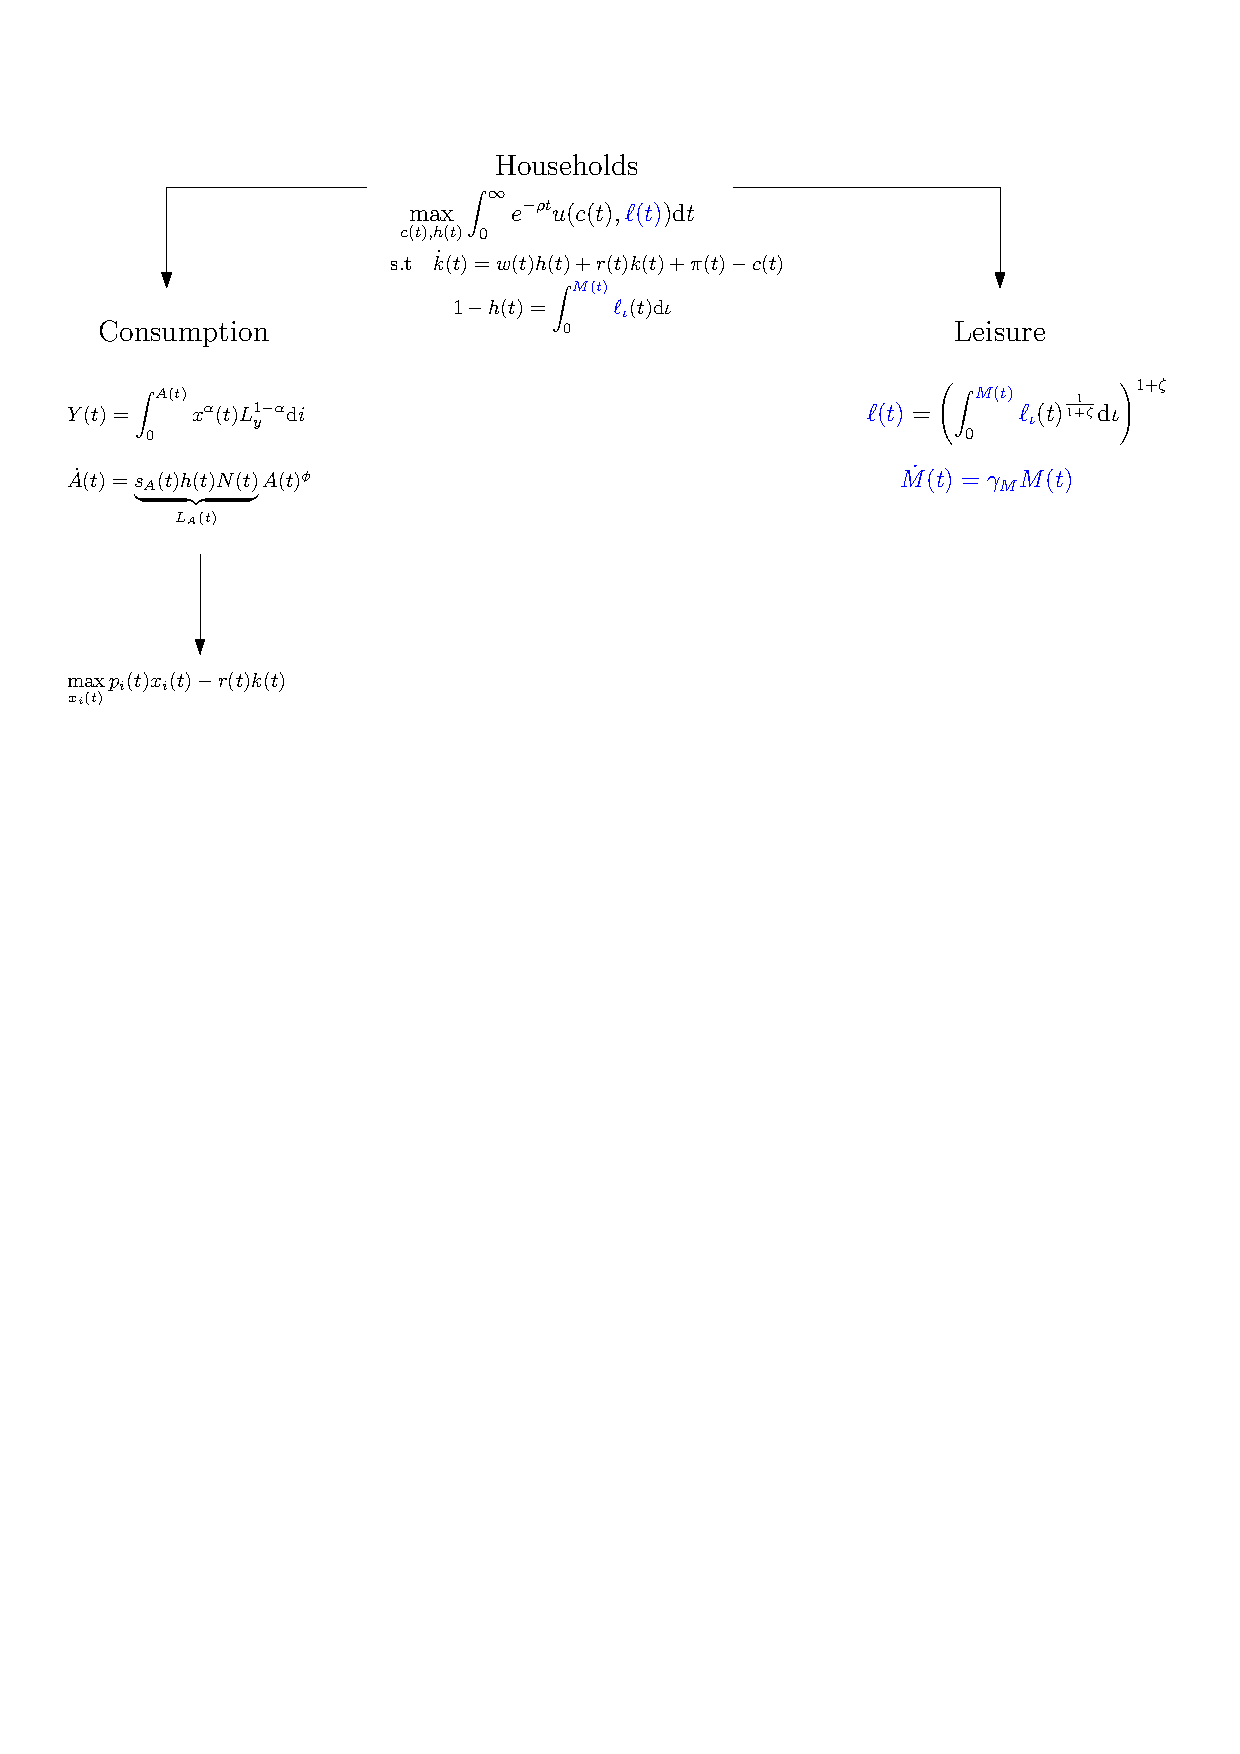
\includegraphics[width = 0.7\textwidth]{Presentation01/Figures/Mod1.pdf}
        \caption{Model Overview}
    \end{figure}
\end{frame}

\begin{frame}{Taking Stock}
\begin{itemize}
    \item On a BGP the growth rates are \\ \vspace{0.5cm}
    \begin{table}[htb]
        \centering
        \begin{tabular}{lcc} \hline
             Object & Growth & Type \\
             \hline\hline
             $N(t)$ & $n$ & Exogenous \\ 
             $M(t)$ & $\gamma_M$ & Exogenous \\ 
             $h(t)$ & $\textcolor{blue}{-\zeta \gamma_M}$ & Endogenous \\ 
             $A(t)$ & $\dfrac{n\textcolor{blue}{-\zeta\gamma_M}}{1-\phi}$ & Endogenous \\ 
             $c(t)$ &  $\dfrac{n\textcolor{blue}{-\zeta\gamma_M}}{1-\phi}$ & Endogenous \\ 
             \hline\hline
        \end{tabular}
        \caption{Growth Rates}
    \end{table}
    \item Welfare? Ambiguous. Utility from leisure vs. consumption. 
    \end{itemize}
\end{frame}

\subsection{Static Model}


\begin{frame}{Endogenous Leisure Technology}
    \begin{figure}
        \centering
        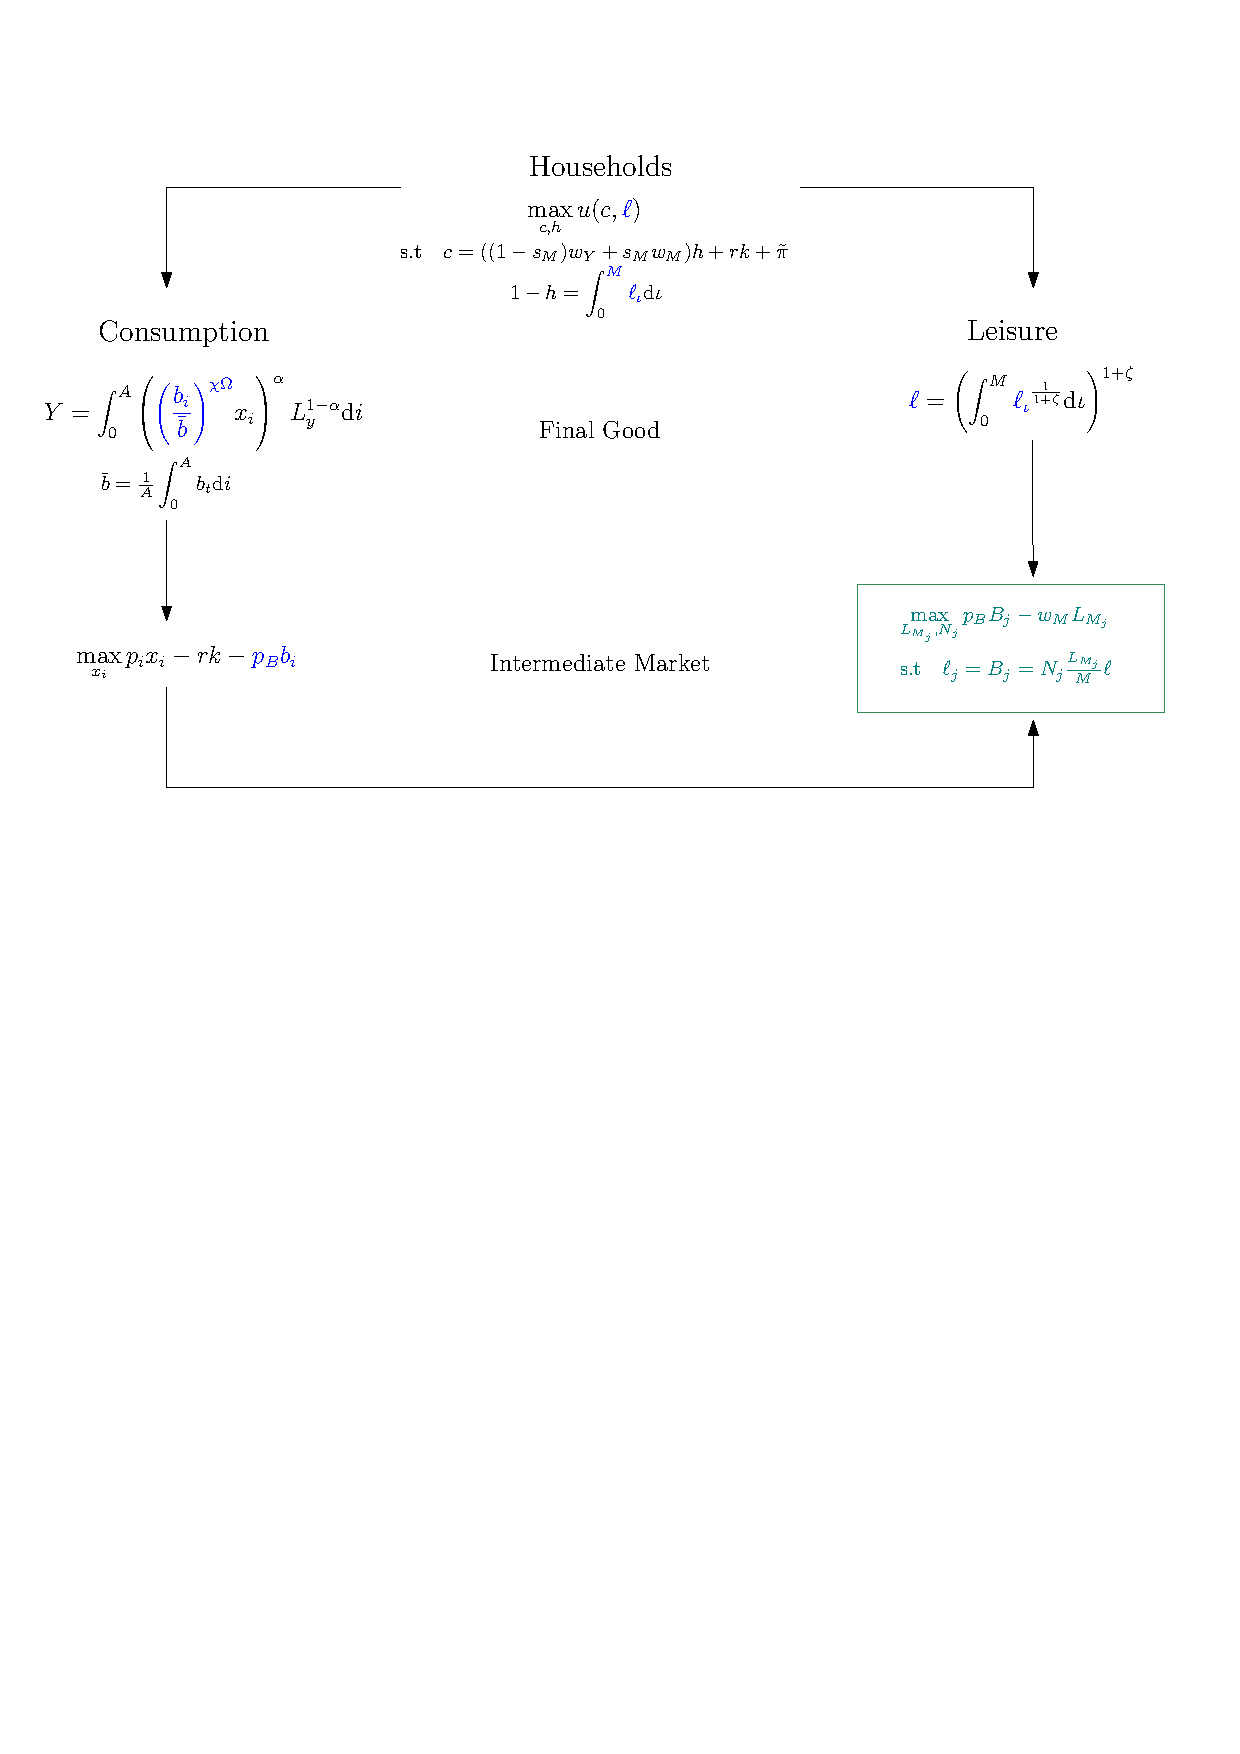
\includegraphics[width = 0.7\textwidth]{Presentation01/Figures/Mod2.pdf}
        \caption{Model Overview}
    \end{figure}
\end{frame}

\section{Results}

\begin{frame}{Taking the Model to the Data}
\begin{figure}
    \centering    
    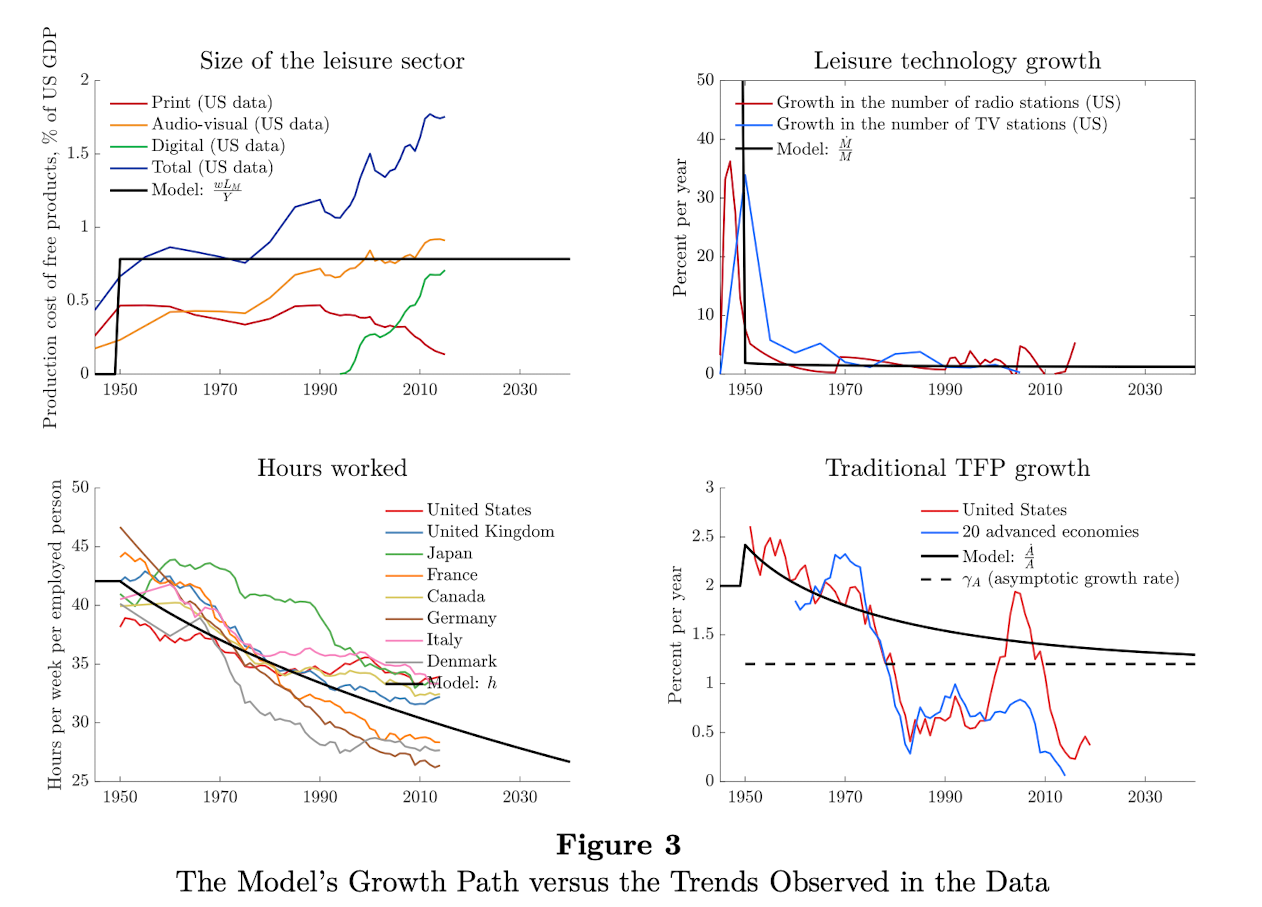
\includegraphics[width=0.7\textwidth]{Presentation01/Figures/ModTrends.png}
\end{figure}  
\end{frame}

\section{Conclusions}

\begin{frame}{Conclusions}

\begin{itemize}
    \item The big achievement of this paper is that distinguish between traditional products and leisure-directed products. 
    \item The way consumers interact with leisure products brings together macroeconomic trends that were studied separately. 
\end{itemize}    
\pause 
Some of my takes... 
\begin{itemize}
    \item It's a milestone to start differentiating consumption products and leisure products. 
    \item There is a big gap between the model and the data. 
    \item All the results are mechanical
    \begin{enumerate}
        \item Still work to do on the law of motion of $M(t)$. The economics behind are still raw. 
        \item What about creative destruction? 
    \end{enumerate}
\end{itemize}
\end{frame}

\begin{frame}
\begin{center}    
    \Huge{Thank You}
\end{center}
\end{frame}



\begin{frame}{Motivational Trends}\label{p1:Mot}
    \begin{figure}
    \centering    
    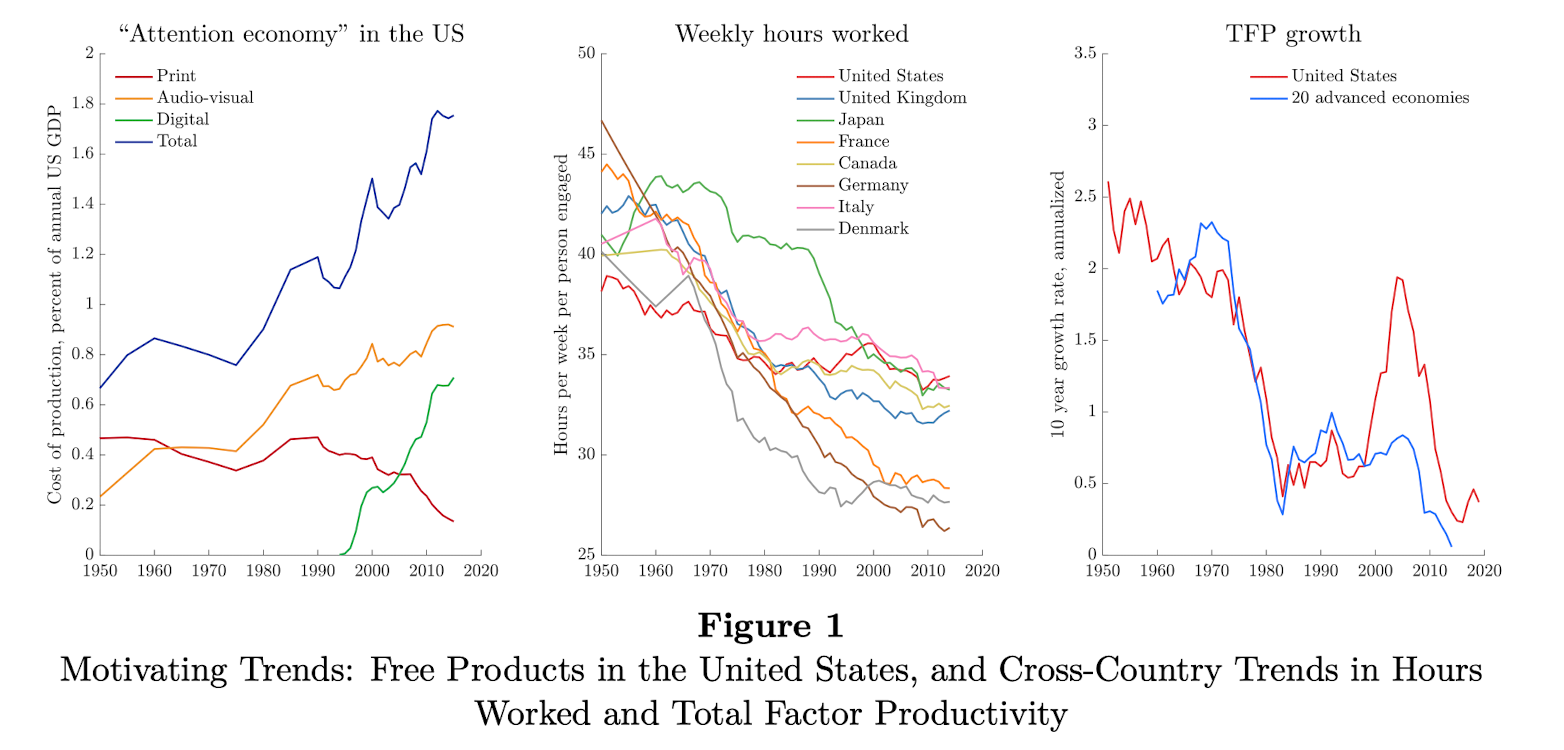
\includegraphics[width=\textwidth]{Presentation01/Figures/MotFacts.png}
\end{figure}
\hyperlink{p1:Int}{\beamerbutton{Back}}

\end{frame}



\end{document}

